\section{Background}
% for the intro put listings into Matlab mode
\lstset{language=Matlab}

\mixten is implemented on top of several existing \matlab compiler tools.
The overall structure is given in \figref{Fig:Overview},  where the new
parts are indicated by the shaded boxes, and future work is indicated by
dashed boxes.     

\begin{figure}[htbp] 
\begin{center}
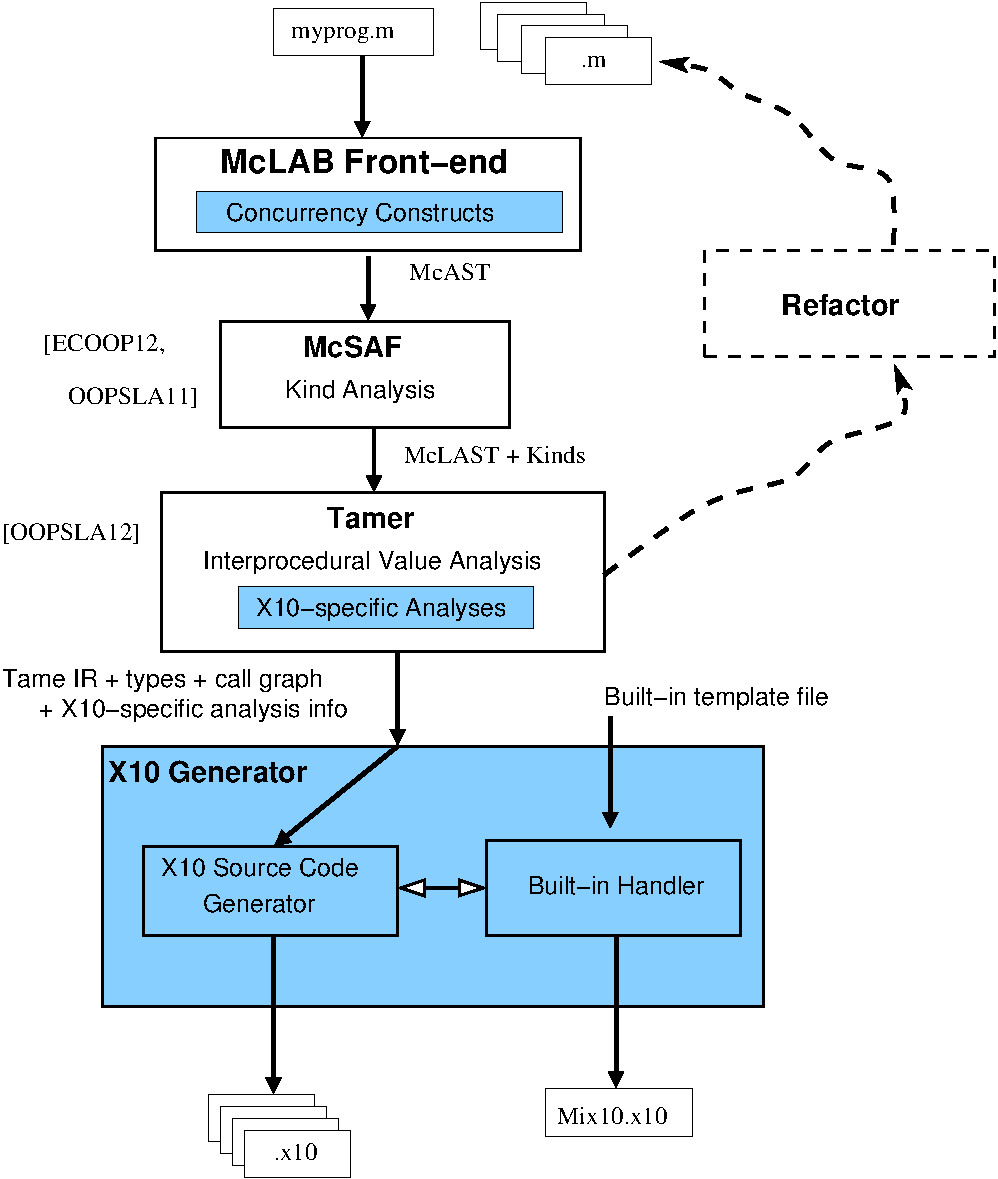
\includegraphics[width=3.2in]{Figures/overview.pdf} 
\caption {Overview of \mixten structure}\label{Fig:Overview}
\end{center}
\end{figure}

As illustrated at the top of the figure, a \matlab programmer only needs
to provide an entry-point \matlab function (called \texttt{myprog.m} in
this example),  plus a collection of other
\matlab functions and libraries (directories of functions)
which may be called, directly or indirectly, by the entry point.   The
programmer may also specify the types and/or shapes of the input
parameters to the entry-point function.   As shown at the bottom of the
figure, our \mixten compiler automatically produces a collection of
\xten output files which contain the generated \xten code for all
reachable \matlab functions, plus one \xten file called
\texttt{mix10.x10} which contains generated and specialized \xten code
for the required builtin \matlab functions.  Thus, from the \matlab
programmer's point of view,  the \mixten compiler is quite simple to
use.

\matlab is actually quite a complicated language to compile,  starting
with its rather unusual syntax,  which cannot be parsed with standard
LALR techniques.  There are several issues that must be dealt with
including distinguishing places where white space and new line characters have 
syntactic meaning, and filling in missing \lstinline!end! keywords,
which are sometimes optional.   The \mclab front-end
handles the parsing of \matlab through a two step process.  There is a
pre-processing step which translates \matlab programs to a cleaner
subset, called \textit{Natlab}, which has a grammar that can be
expressed cleanly for a LALR parser.    The \mclab front-end delivers a
high-level AST based on this cleaner grammar.  
\begin{comment}
 For the \mixten project
we have extended the front-end to handle \xten- inspired concurrency
constructs,  exposed in the \matlab program as extended comments.
\end{comment}

After parsing,  the next major phase of \mixten uses the \mcsaf
framework~\cite{McSAFecoop12,JesseThesis} to disambiguate identifiers
using \textit{kind analysis}~\cite{KindAnalysis}, which determines if an
identifier refers to a \textit{variable} or a \textit{named function}.
This is required because the syntax of \matlab does not distinguish
between variables and functions. For example, the expression
\lstinline!a(i)! could refer to four different computations,
\lstinline!a! could be an array or a function,  and \lstinline!i! could
refer to the builtin function for the imaginary value $i$,  or it could
refer to a variable \lstinline!i!.    The \mcsaf framework also
simplifies the AST, producing a lower-level AST which is more amenable
to subsequent analysis.

The next major phase is the Tamer~\cite{TamerPaper}, which is a key
component for any tool which statically compiles \matlab.  The Tamer
generates an even more defined AST called \textit{Tamer IR}, as well as
performing key interprocedural analyses to determine both the call graph
and an estimate of the base type and shape of each variable, at each
program point.   The call graph is needed to determine which files
(functions) need to be compiled,  and the type and shape information is
very important for generating reasonable code when the target language
is statically typed, as is the case for \xten.  

\begin{comment}
The Tamer may find dynamic \matlab features which cannot be statically
compiled, in which case it flags that feature as not tame,  and the
ultimate goal is to support a refactoring tool which would aid the
programmer to restructure their input \matlab program in order to
eliminate the wild feature.
\end{comment}

The Tamer also provides an extensible \textit{interprocedural value
analysis} and an interprocedural analysis framework that extends the
intraprocedural framework provided by \mcsaf.   Any static backend will
use the standard results of the Tamer,  but is also likely to implement
some target-language-specific analyses which estimate properties useful
for generating code in a specific target language. Currently, we have
implemented two analyses : (1) An analysis for determining if a \matlab
variable is \textit{real} or \textit{complex} to enable support for
complex numbers in \mixten and other \matlab compilers based on \mclab;
and (2) \emph{IntegerOkay} analysis to identify which variables can be
safely declared to be of an integer type (\texttt{Int} or \texttt{Long})
instead of the default type \texttt{Double}.  

For the purposes of \mixten, the output of the Tamer is a low-level,
well-structured AST, which along with key analysis information about the
call graph,  the types and shapes of variables, and X10-specific
information.   These Tamer outputs are provided to the code generator,
which generates \xten code, and which is the main focus of this thesis.

The \xten source code generator actually gets inputs from two places.  It uses
the Tamer IR it receives from the the Tamer to drive the code generation,  but
for expressions referring to built-in \matlab functions it interacts with the
\textit{Built-in Handler} which used the built-in template file we provide.  We
describe the functioning of the
built-in handler in \chapref{chap:Builtins}. 

\chapref{chap:Arrays} concentrates on generating efficient code for \matlab
arrays.  \chapref{chap:CodegenSeq} describes the code generation strategy for
the sequential core of \matlab, while \chapref{chap:CodegenCon} describes our
strategy to generate parallel \xten code for \matlab \texttt{parfor} construct,
and introducing \xten like concurrency constructs in \matlab. The focus of this
thesis is to address challenges in generating \emph{efficient} \xten code whose
performance is comparable to state-of-the-art tools that generate more
traditional imperative languages like C and Fortran.

\section{High-level Design of the \mixten Compiler}

The \mixten code generator is the key component which makes the
translation from the Tamer IR, which is based on \matlab programming
constructs and semantics,  to \xten.  The overall structure of the
\mixten code generator is given in \figref{Fig:x10}.

\begin{figure}[htbp] 
\begin{center}
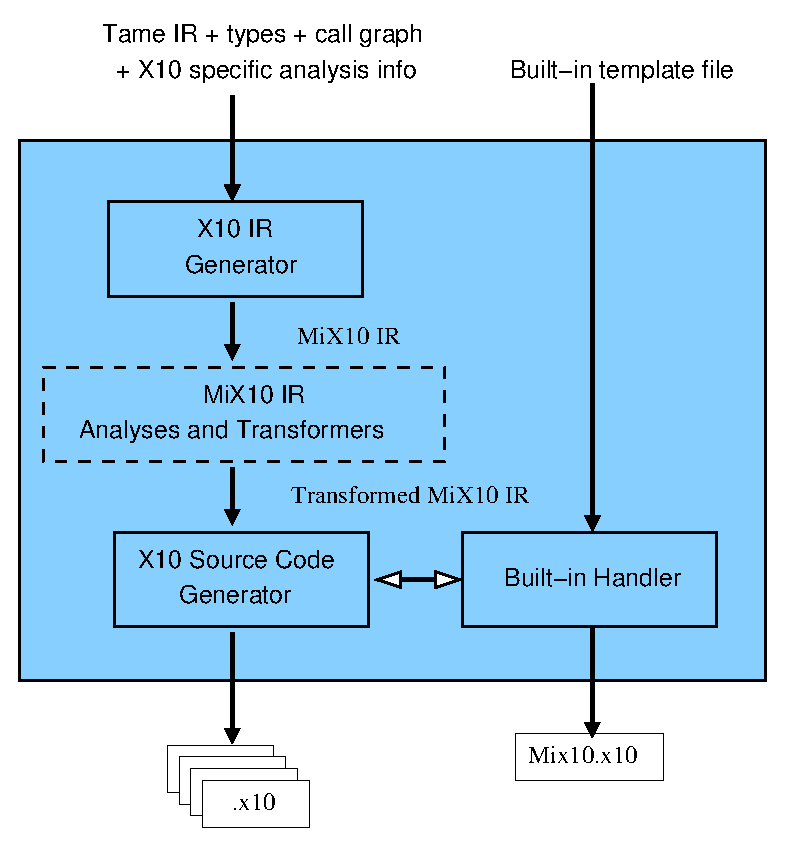
\includegraphics[width=3.2in]{Figures/x10.eps} 
\caption{Structure of the MiX10 code generator}\label{Fig:x10}
\end{center}
\end{figure}

 The input to to \mixten compiler is the call graph generated by Tamer and the
Tame IR annotated with the necessary analysis information like \emph{shape},
\emph{iscomplex}, and \emph{type} and \emph{IntegerOkay}.  Rather than do a
direct code generation to \xten source code, \mixten translates the Tamer IR to
\mixten IR, a general and extensible IR, designed by us, to represent \xten.
This translation is done by the \xten IR generator module of \mixten. Finally,
with the inputs from the builtin handler and the \xten IR generator (after the
\xten specific analyses and transformations have been done), the \xten source
code generator generates the resultatnt \xten source code.

\subsection{The \mixten Intermediate Representation}

The \mixten IR is a low-level, three address like intermediate representation
that is similar in design to the Tamer IR and abstracts the \xten constructs
while capturing the static information required to generate the \xten source
code.
We have implemented the IR using JastAdd~\cite{ekman04,jastaddurl}, which allows
us to easily add new AST nodes by simply extending the JastAdd
specification grammar.

There are three important reasons to use an IR, instead of directly generating the
\xten code: \begin{itemize} 

\item There are potentially two places that
optimizations and transformations may happen:  either at the Tamer IR level or
at the \mixten IR level.  It is our intent to put any analysis or transformation
that is not \xten-specific into the Tamer IR, so that other back-ends can
benefit from those improvements.   However, optimizations and  transformations
that are specific to \xten programming constructs (such as points and regions)
and semantics will need to be done on the \mixten IR. Although we currently do
not transform the \mixten IR very much, the ultimate goal is to support a
variety of analyses and transformations that can be used to: (1) produce more
efficient \xten code, and (2) produce more readable \xten code.  

\item There are \xten constructs that can be pretty
printed to be of different kinds, for example the \xten arrays, which can either
be simple arrays, region arrays or specialized region arrays, and \xten for loop
which can either be C-like for loop or an iterator over a \texttt{LongRange}
(used in generated code for \texttt{parfor} loop). It allows to abstract the
vital information for a construct while leaving the actual syntax to the source
code generator. This makes it easier to add \xten specific analyses and
transformations, and makes it easy to update the compiler whenever a new or
improved variation of a construct is added. 

\item \mixten IR can also be used as a convenient place to insert
instrumentation code for the generated \xten code.

\end{itemize}   

Appendix \ref{chap:irgrammar} provides the JastAdd implementation of the \mixten IR
grammar.

%As shown in \figref{Fig:x10}, the \xten source code generator actually
%gets inputs from two places.   It uses the \mixten IR to drive the code
%generation,  but for expressions referring to built-in \matlab functions
%it interacts with the \textit{Built-in Handler}.  In 
%\chapref{chap:Builtins}, we discuss this process in in more detail, and in
%the subsequent chapters,  \chapref{chap:CodegenSeq} and
%\chapref{chap:CodegenCon} we address the source code
%generation for the key \xten constructs.
%

